\begin{frame}
\begin{footnotesize}
\frametitle{Példa: Sűrű / ritka gráfok}
\note{Everything you want}

\begin{columns}
\begin{column}{0.5\textwidth}
Sűrű gráf:
\begin{center}
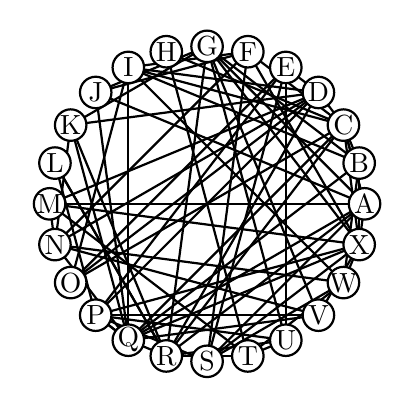
\begin{tikzpicture}[scale=2]
\coordinate (A) at (2.00000,1.00000);
\coordinate (B) at (1.96593,1.25882);
\coordinate (C) at (1.86603,1.50000);
\coordinate (D) at (1.70711,1.70711);
\coordinate (E) at (1.50000,1.86603);
\coordinate (F) at (1.25882,1.96593);
\coordinate (G) at (1.00000,2.00000);
\coordinate (H) at (0.74118,1.96593);
\coordinate (I) at (0.50000,1.86603);
\coordinate (J) at (0.29289,1.70711);
\coordinate (K) at (0.13397,1.50000);
\coordinate (L) at (0.03407,1.25882);
\coordinate (M) at (0.00000,1.00000);
\coordinate (N) at (0.03407,0.74118);
\coordinate (O) at (0.13397,0.50000);
\coordinate (P) at (0.29289,0.29289);
\coordinate (Q) at (0.50000,0.13397);
\coordinate (R) at (0.74118,0.03407);
\coordinate (S) at (1.00000,0.00000);
\coordinate (T) at (1.25882,0.03407);
\coordinate (U) at (1.50000,0.13397);
\coordinate (V) at (1.70711,0.29289);
\coordinate (W) at (1.86603,0.50000);
\coordinate (X) at (1.96593,0.74118);
\draw[thick] (B) -- (Q);
\draw[thick] (G) -- (V);
\draw[thick] (R) -- (U);
\draw[thick] (M) -- (X);
\draw[thick] (P) -- (P);
\draw[thick] (G) -- (U);
\draw[thick] (N) -- (M);
\draw[thick] (B) -- (I);
\draw[thick] (F) -- (N);
\draw[thick] (Q) -- (N);
\draw[thick] (A) -- (S);
\draw[thick] (N) -- (V);
\draw[thick] (X) -- (B);
\draw[thick] (B) -- (X);
\draw[thick] (J) -- (A);
\draw[thick] (T) -- (R);
\draw[thick] (F) -- (X);
\draw[thick] (N) -- (W);
\draw[thick] (V) -- (Q);
\draw[thick] (Q) -- (C);
\draw[thick] (R) -- (G);
\draw[thick] (Q) -- (R);
\draw[thick] (J) -- (F);
\draw[thick] (M) -- (D);
\draw[thick] (C) -- (H);
\draw[thick] (G) -- (A);
\draw[thick] (T) -- (U);
\draw[thick] (P) -- (Q);
\draw[thick] (H) -- (T);
\draw[thick] (P) -- (U);
\draw[thick] (C) -- (D);
\draw[thick] (S) -- (X);
\draw[thick] (S) -- (F);
\draw[thick] (X) -- (A);
\draw[thick] (I) -- (W);
\draw[thick] (I) -- (O);
\draw[thick] (I) -- (Q);
\draw[thick] (A) -- (C);
\draw[thick] (D) -- (O);
\draw[thick] (C) -- (A);
\draw[thick] (G) -- (J);
\draw[thick] (V) -- (X);
\draw[thick] (I) -- (D);
\draw[thick] (R) -- (D);
\draw[thick] (R) -- (C);
\draw[thick] (O) -- (E);
\draw[thick] (L) -- (P);
\draw[thick] (L) -- (R);
\draw[thick] (Q) -- (X);
\draw[thick] (W) -- (T);
\draw[thick] (E) -- (P);
\draw[thick] (K) -- (R);
\draw[thick] (S) -- (P);
\draw[thick] (U) -- (E);
\draw[thick] (V) -- (P);
\draw[thick] (R) -- (R);
\draw[thick] (E) -- (D);
\draw[thick] (B) -- (G);
\draw[thick] (M) -- (T);
\draw[thick] (N) -- (D);
\draw[thick] (D) -- (K);
\draw[thick] (X) -- (C);
\draw[thick] (C) -- (I);
\draw[thick] (N) -- (K);
\draw[thick] (A) -- (Q);
\draw[thick] (G) -- (X);
\draw[thick] (E) -- (S);
\draw[thick] (M) -- (A);
\draw[thick] (P) -- (X);
\draw[thick] (W) -- (S);
\draw[thick] (F) -- (I);
\draw[thick] (M) -- (M);
\draw[thick] (R) -- (A);
\draw[thick] (Q) -- (K);
\draw[thick] (R) -- (L);
\draw[thick] (Q) -- (P);
\draw[thick] (J) -- (Q);
\draw[thick] (P) -- (D);
\draw[thick] (G) -- (K);
\draw[thick] (W) -- (X);
\draw[thick] (C) -- (B);
\draw[thick] (W) -- (W);
\draw[thick] (F) -- (C);
\draw[thick] (O) -- (C);
\draw[thick] (H) -- (H);
\draw[thick] (W) -- (B);
\draw[thick, fill=white] (A) circle (0.1) node {A};
\draw[thick, fill=white] (B) circle (0.1) node {B};
\draw[thick, fill=white] (C) circle (0.1) node {C};
\draw[thick, fill=white] (D) circle (0.1) node {D};
\draw[thick, fill=white] (E) circle (0.1) node {E};
\draw[thick, fill=white] (F) circle (0.1) node {F};
\draw[thick, fill=white] (G) circle (0.1) node {G};
\draw[thick, fill=white] (H) circle (0.1) node {H};
\draw[thick, fill=white] (I) circle (0.1) node {I};
\draw[thick, fill=white] (J) circle (0.1) node {J};
\draw[thick, fill=white] (K) circle (0.1) node {K};
\draw[thick, fill=white] (L) circle (0.1) node {L};
\draw[thick, fill=white] (M) circle (0.1) node {M};
\draw[thick, fill=white] (N) circle (0.1) node {N};
\draw[thick, fill=white] (O) circle (0.1) node {O};
\draw[thick, fill=white] (P) circle (0.1) node {P};
\draw[thick, fill=white] (Q) circle (0.1) node {Q};
\draw[thick, fill=white] (R) circle (0.1) node {R};
\draw[thick, fill=white] (S) circle (0.1) node {S};
\draw[thick, fill=white] (T) circle (0.1) node {T};
\draw[thick, fill=white] (U) circle (0.1) node {U};
\draw[thick, fill=white] (V) circle (0.1) node {V};
\draw[thick, fill=white] (W) circle (0.1) node {W};
\draw[thick, fill=white] (X) circle (0.1) node {X};
\end{tikzpicture}
\end{center}

\end{column}

\begin{column}{0.5\textwidth}
Ritka gráf:
\begin{center}
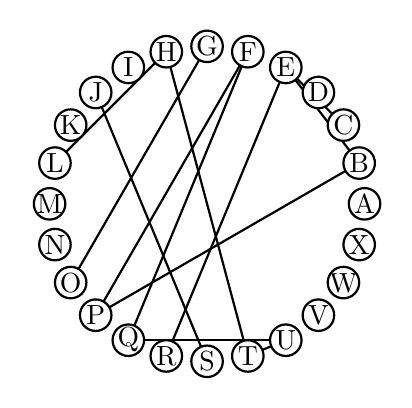
\begin{tikzpicture}[scale=2]
\coordinate (A) at (2.00000,1.00000);
\coordinate (B) at (1.96593,1.25882);
\coordinate (C) at (1.86603,1.50000);
\coordinate (D) at (1.70711,1.70711);
\coordinate (E) at (1.50000,1.86603);
\coordinate (F) at (1.25882,1.96593);
\coordinate (G) at (1.00000,2.00000);
\coordinate (H) at (0.74118,1.96593);
\coordinate (I) at (0.50000,1.86603);
\coordinate (J) at (0.29289,1.70711);
\coordinate (K) at (0.13397,1.50000);
\coordinate (L) at (0.03407,1.25882);
\coordinate (M) at (0.00000,1.00000);
\coordinate (N) at (0.03407,0.74118);
\coordinate (O) at (0.13397,0.50000);
\coordinate (P) at (0.29289,0.29289);
\coordinate (Q) at (0.50000,0.13397);
\coordinate (R) at (0.74118,0.03407);
\coordinate (S) at (1.00000,0.00000);
\coordinate (T) at (1.25882,0.03407);
\coordinate (U) at (1.50000,0.13397);
\coordinate (V) at (1.70711,0.29289);
\coordinate (W) at (1.86603,0.50000);
\coordinate (X) at (1.96593,0.74118);
\draw[thick] (T) -- (H);
\draw[thick] (Q) -- (U);
\draw[thick] (P) -- (F);
\draw[thick] (S) -- (J);
\draw[thick] (C) -- (E);
\draw[thick] (B) -- (P);
\draw[thick] (G) -- (O);
\draw[thick] (Q) -- (F);
\draw[thick] (E) -- (B);
\draw[thick] (H) -- (L);
\draw[thick] (E) -- (R);
\draw[thick] (T) -- (U);
\draw[thick, fill=white] (A) circle (0.1) node {A};
\draw[thick, fill=white] (B) circle (0.1) node {B};
\draw[thick, fill=white] (C) circle (0.1) node {C};
\draw[thick, fill=white] (D) circle (0.1) node {D};
\draw[thick, fill=white] (E) circle (0.1) node {E};
\draw[thick, fill=white] (F) circle (0.1) node {F};
\draw[thick, fill=white] (G) circle (0.1) node {G};
\draw[thick, fill=white] (H) circle (0.1) node {H};
\draw[thick, fill=white] (I) circle (0.1) node {I};
\draw[thick, fill=white] (J) circle (0.1) node {J};
\draw[thick, fill=white] (K) circle (0.1) node {K};
\draw[thick, fill=white] (L) circle (0.1) node {L};
\draw[thick, fill=white] (M) circle (0.1) node {M};
\draw[thick, fill=white] (N) circle (0.1) node {N};
\draw[thick, fill=white] (O) circle (0.1) node {O};
\draw[thick, fill=white] (P) circle (0.1) node {P};
\draw[thick, fill=white] (Q) circle (0.1) node {Q};
\draw[thick, fill=white] (R) circle (0.1) node {R};
\draw[thick, fill=white] (S) circle (0.1) node {S};
\draw[thick, fill=white] (T) circle (0.1) node {T};
\draw[thick, fill=white] (U) circle (0.1) node {U};
\draw[thick, fill=white] (V) circle (0.1) node {V};
\draw[thick, fill=white] (W) circle (0.1) node {W};
\draw[thick, fill=white] (X) circle (0.1) node {X};
\end{tikzpicture}
\end{center}

\end{column}
\end{columns}

Erre a két gráfra nézzünk gráfalgoritmusokat:
\begin{itemize}
\item Legnagyobb független csúcshalmaz.
\item Csúcsszínezés.
\item Stb...
\end{itemize}

Mindkét gráfban ugyanannyi csúcs van, ezért ha szomszédossági mátrixukkal adjuk meg őket, akkor
ugyanakkora lesz az input mérete, azonban a 2. gráfban a fenti kérdésekre elég hamar választ
tudunk adni.
\end{footnotesize}
\end{frame}

